\chapter{Technologies Used}
\label{chap:Chapter 3 title}
The adoption of the DevOps approach largely relies on the automation of communication between the various required tools, thus allowing us to benefit from the previously described functionalities. The choice of tools for each stage of our DevOps pipeline, such as continuous integration and continuous deployment, depends on specific criteria related to our needs. Consequently, this comparative study aims to reinforce the selection of tools that we have implemented for the integration of Green IT into DevOps practices.

\newpage


\section{Application Containerization}
In this section, we will delve into our problem by examining the fundamental principles of traditional virtualization and containerization. Our aim is to provide a clear description of these concepts and explain the relationships between them.

\subsection{Virtualization}
Virtualization involves creating a virtual version of a device or resource, such as an operating system, server, storage device, or network resource. It allows for the abstraction of physical resources, representing them independently of their physical equivalents. Each virtual element, such as a disk, network interface, local network, switch, processor, or memory, is associated with a physical resource in a computer system. Thus, virtual machines hosted by the host machine are considered applications that require allocation or distribution of the host's resources. There are various types of virtualization, each corresponding to a specific use case:

\begin{itemize}
    \item \textbf{System Virtualization} is a server virtualization technique that uses a hypervisor to allow the host machine to run multiple virtual instances simultaneously. These virtual instances are commonly referred to as virtual machines (VMs), while the hypervisor is known as the virtual machine monitor (VMM), responsible for managing the VMs.
    \item \textbf{Application Virtualization} differs from system virtualization by using a virtualization layer in the form of an application. This application creates virtual instances and isolates them from the specifics of the host machine, such as its architecture or operating system. This approach allows developers to avoid creating multiple versions of their software to run in different environments. Common application virtual machines include the JVM (Java Virtual Machine) and containers.
\end{itemize}

\subsection{Containerization}
Container-based virtualization, also known as containerization, offers an alternative to system virtualization. This approach directly leverages kernel features to create isolated virtual environments called containers. Containers use control groups (cgroups) and namespaces provided by the operating system kernel. Namespaces allow for controlling and limiting the resources used by a process, while cgroups manage the resources of a group of processes. Thus, a container provides the necessary resources to run applications in isolation, as if they were the only processes running on the host machine's operating system.

Containers offer advantages such as scalable, modular, and loosely coupled application development. The need to create portable deliverables independent of development or production environments has become a standard. The term "container" emerged to refer to an application independent of the system, represented as a box containing all the dependencies necessary for its proper functioning.

\subsection{Containerization vs Virtualization}
Containers have an intrinsically smaller footprint than virtual machines and require less startup time. This means that more containers can run on the same computing capacity compared to a single virtual machine. This improvement in server efficiency reduces costs associated with servers and licenses. In simple terms, containerization allows applications to be developed once and run anywhere. This portability is crucial for streamlining the development process and ensuring compatibility with different service providers.

Figure \ref{fig:container_vs_vm} illustrates the distinction between container architecture and virtual machine architecture.

\begin{figure}[h]
    \centering
    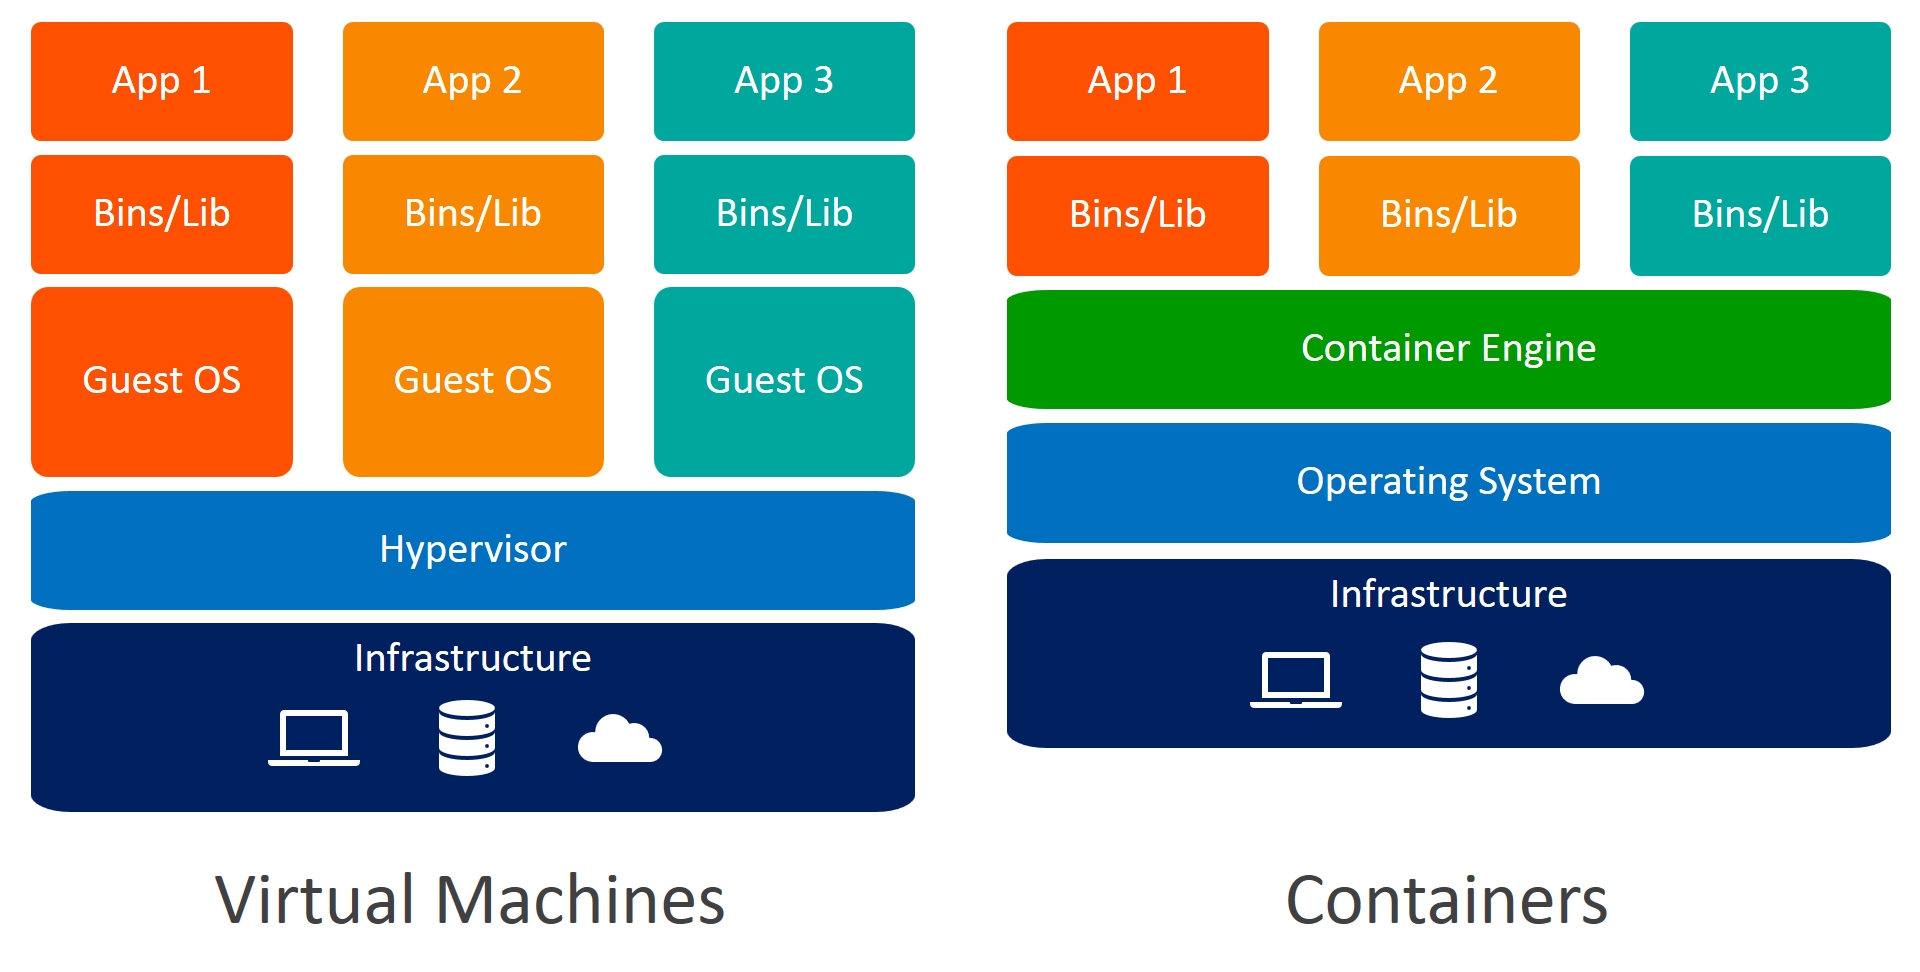
\includegraphics[width=16cm]{Figures/containers-vs-vms.jpg}
    \caption{Comparison between Container and Virtual Machine Architectures}
    \label{fig:container_vs_vm}
\end{figure}

\subsection{Containerization Technologies}
There are several containerization tools available in the market. We conducted a comparison to select the most suitable one.

\begin{table}[h]
    \centering
    \begin{tabular}{|p{4cm}|p{4cm}|p{4cm}|p{4cm}|}
        \hline
        \textbf{Technology} & \textbf{Principle} & \textbf{Market Position} & \textbf{Documentation/ Complexity} \\
        \hline
        \textbf{Docker} & A container contains a single process; multiple containers can be connected to form an application. & Market leader, widely used by major online service providers (e.g., Netflix, Spotify) & Official documentation is available; community-driven tutorials and resources are abundant. Known for its simplicity.\\
        \hline
        \textbf{Podman} & A container contains a single process; multiple containers can be connected to form an application. & Increasingly popular, supported by major enterprises like Google and Red Hat. Acquired by Red Hat in May 2018. & Limited documentation, somewhat difficult due to lack of resources but highly modular and compatible with ancillary tools.\\
        \hline
        \textbf{LXC/LXD} & Isolation of an entire application within a complete Linux environment (similar to a VM). & Established since 2008, the only one closely resembling a VM. Isolated but with an active community. & Limited documentation; most information is posted on Ubuntu community forums. \\
        \hline
    \end{tabular}
    \caption{Comparison of Containerization Tools}
    \label{tab:container_tools_comparison}
\end{table}

The analysis presented in Table \ref{tab:container_tools_comparison} highlights the significance of Docker in the market. Docker stands out as the most universal solution in terms of image compatibility and offers numerous additional advantages. It simplifies the creation and management of containers, facilitates the design and construction of images, and enables easy distribution and version control of these images. Thus, Docker plays a crucial role in streamlining and enhancing containerization processes.

\section{Introduction to Docker}
Docker uses a client-server architecture. The Docker client talks to the Docker daemon, which does the heavy lifting of building, running, and distributing your Docker containers. The Docker client and daemon can run on the same system, or you can connect a Docker client to a remote Docker daemon. The Docker client and daemon communicate using a REST API, over UNIX sockets or a network interface. Another Docker client is Docker Compose, that lets you work with applications consisting of a set of containers.
\newpage
\begin{itemize}
  \item \textbf{Docker Daemon (\textit{dockerd}):} Responsible for handling Docker API requests and managing various Docker objects such as images, containers, networks, and volumes. Listens for incoming requests and executes them accordingly. Can interact with other daemons to manage Docker services across different environments.
  
  \item \textbf{Docker Client (\textit{docker}):} Primary interface for Docker users to interact with the Docker ecosystem. Users issue commands through the Docker client (e.g., \texttt{docker run}), which are communicated to the daemon for execution. Utilizes the Docker API for communication and can connect with multiple daemons for managing Docker instances.
  
  \item \textbf{Docker Registries:} Facilitate storage and distribution of containerized applications. Docker Hub is a public registry accessible to all users, while private registries can be set up for hosting proprietary or sensitive images. Commands like \texttt{docker pull} or \texttt{docker run} fetch required images from the configured registry, and \texttt{docker push} uploads images to the designated registry for sharing or backup purposes.
\end{itemize}

\begin{figure}[h]
  \centering
  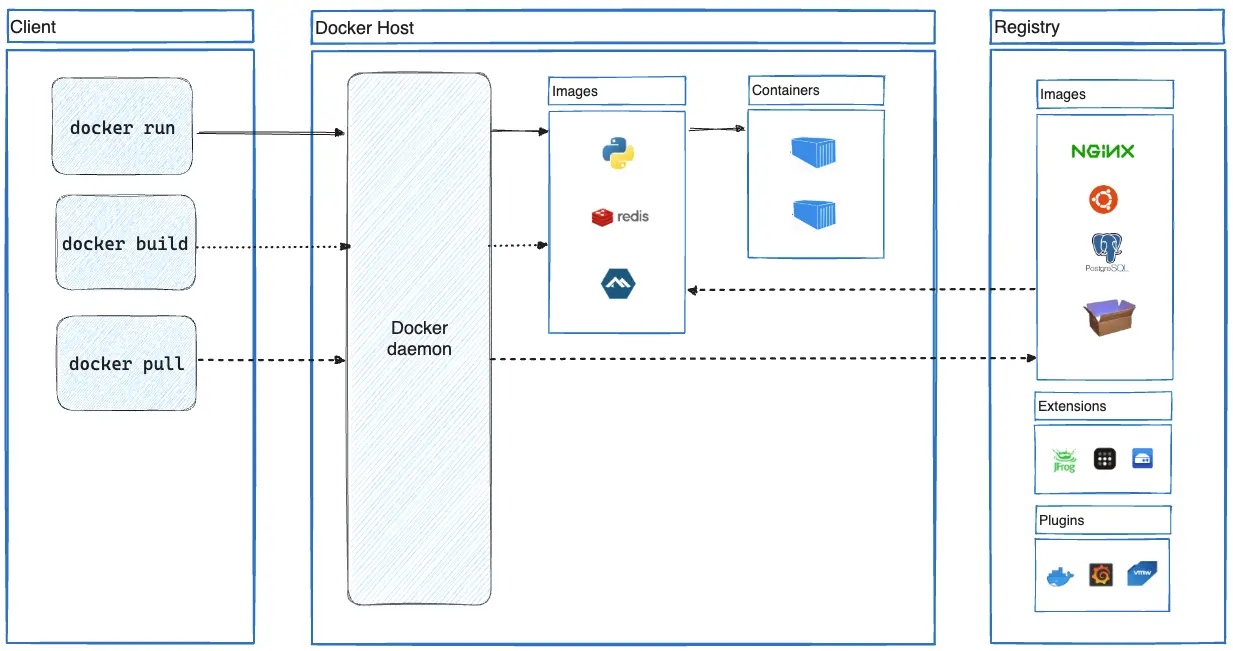
\includegraphics[width=\textwidth]{Figures/docker-architecture.png}
  \caption{Docker Architecture}
  \label{fig:container_architecture}
\end{figure}

\section{Container Orchestration}

Container orchestration involves automating much of the operational tasks required to run containerized workloads and services. This encompasses various aspects that software teams need to manage the lifecycle of a container, such as provisioning, deployment, scaling (both up and down), network management, and load balancing. Container orchestration simplifies and optimizes container management by providing tools and features to effectively coordinate different container instances and associated resources. This facilitates the deployment and management of complex and scalable containerized applications in production environments.

\subsection{Why Orchestration is Necessary}

The ability to create containers has existed for several decades but became widely accessible in 2008 when Linux integrated container functionality into its kernel. However, widespread adoption of containers took off with the introduction of Docker, an open-source containerization platform, in 2013. Docker became so popular that the terms "Docker containers" and "containers" are often used interchangeably.

Containers have become the de facto computing units for modern cloud-native applications due to their small size, resource efficiency, and portability compared to virtual machines (VMs). Containerized microservices or serverless functions are particularly prevalent in these applications. Manually deploying and managing a small number of containers is relatively easy. However, in most organizations, the number of containerized applications is rapidly increasing, making large-scale management impossible without automation. This is where container orchestration comes into play.

Container orchestration provides essential automation for managing a large number of containerized applications. This significantly reduces the effort and complexity associated with managing this application fleet. By automating operations, orchestration facilitates an agile or DevOps approach, allowing development teams to rapidly deploy new features and capabilities.

The automation provided by orchestration enhances many inherent benefits of containerization. For example, it enables automated host selection and efficient resource allocation based on declarative configuration, thereby maximizing the utilization of computing resources. Additionally, orchestration provides automated monitoring of container health status and can move containers as needed to maximize availability.

In summary, container orchestration brings essential automation to effectively manage a large number of containerized applications. It facilitates rapid and iterative development cycles, allowing teams to release new features and capabilities more quickly. Furthermore, orchestration can enhance and extend the benefits of containerization through advanced features such as resource management and automated monitoring.

\subsection{Kubernetes Container Orchestration}

Kubernetes is a powerful and popular container orchestration platform that enables enterprises to provide a highly productive PaaS for developing cloud-native applications. With Kubernetes, development teams can focus on coding and innovation, while container infrastructure and operations are managed automatically and efficiently. Kubernetes' advantages over other orchestration solutions (such as Docker Swarm, Apache Mesos, OpenShift, AWS Fargate) largely stem from its various more comprehensive and sophisticated features in several areas, including:

\begin{itemize}
    \item \textbf{Container Deployment:} Kubernetes deploys a specified number of containers on a given host and maintains them in the desired state.
    \item \textbf{Rollouts:} A rollout is a modification to a deployment. Kubernetes allows launching, pausing, resuming, or canceling deployments.
    \item \textbf{Service Discovery:} Kubernetes can automatically expose a container to the internet or other containers using a DNS name or IP address.
    \item \textbf{Storage Provisioning:} Developers can configure Kubernetes to mount local or cloud-based persistent storage for containers as needed.
    \item \textbf{Load Balancing and Scaling:} When traffic to a container experiences a high spike, Kubernetes can employ load balancing and scaling to distribute it across the network to ensure stability and performance. (This also saves developers from having to configure a load balancer)
    \item \textbf{Self-healing for High Availability:} When a container fails, Kubernetes can automatically restart or replace it. It can also take containers out of service that do not meet our health check requirements.
    \item \textbf{Multi-cloud Provider Support and Portability:} Kubernetes enjoys broad support from all major cloud providers. This is particularly important for organizations deploying applications in a hybrid or multi-cloud environment.
\end{itemize}

\section{Helm}

\begin{figure}[H]
  \centering
  
\includegraphics[width=5cm]{Figures/helm-logo.png}
  \caption{Helm}
  \label{fig:helm}
\end{figure}

Helm is a package manager for Kubernetes, facilitating the deployment, management, and scaling of applications within a Kubernetes cluster. Helm simplifies complex Kubernetes application deployments by providing a higher level of abstraction through Helm charts. These charts are pre-configured packages of Kubernetes resources.

\subsection{Key Features of Helm}
\begin{itemize}
    \item \textbf{Charts:} Helm uses charts to define, install, and upgrade even the most complex Kubernetes applications. A Helm chart is a collection of files that describe a related set of Kubernetes resources.
    \item \textbf{Releases:} When a chart is deployed, it becomes a release. Helm manages these releases, enabling rollbacks and upgrades.
    \item \textbf{Repositories:} Helm charts can be stored and shared via repositories, making it easy to distribute applications.
    \item \textbf{Templates:} Helm charts support templates, which allow for dynamic and customizable Kubernetes manifests. Templates are written in Go templating syntax.
    \item \textbf{Lifecycle Management:} Helm provides commands to manage the entire lifecycle of applications, from installation and upgrades to rollbacks and deletion.
\end{itemize}

\subsection{Benefits of Using Helm}
\begin{itemize}
    \item \textbf{Simplified Deployments:} Helm abstracts the complexity of Kubernetes configurations, making deployments more straightforward and repeatable.
    \item \textbf{Version Control:} Helm charts allow you to manage versions of your application, enabling easy rollbacks and upgrades.
    \item \textbf{Sharing and Reusability:} Helm charts can be shared across teams and organizations, promoting reusability and standardization.
    \item \textbf{Scalability:} Helm facilitates the management of applications at scale, handling multiple Kubernetes resources efficiently.
\end{itemize}

Helm significantly enhances the Kubernetes experience by providing a robust framework for managing the complexities of application deployment and lifecycle management. It empowers developers to create more consistent and reliable deployments while reducing the potential for human error.


\section{Source Code Management Tools}

Source Code Management (SCM) concerns how software changes are managed. Its primary goal is to accelerate the delivery of quality code changes by development teams. SCM tools enhance tracking, visibility, collaboration, and control throughout the software development lifecycle, allowing developers working on complex projects to be more creative, have more freedom, and options.

By using SCM, source files are protected against anomalies, and all teams can identify who made which changes and at what stage of the process. This promotes transparency and facilitates collaboration among team members.

We conducted a source code manager study to consolidate the choice of the GitLab tool, which is already used by Orange Business, compared to its competitors BitBucket and GitHub.

Table 3.2 summarizes the comparison of the previously presented source code managers:

\begin{table}[h]
  \centering
  \resizebox{\textwidth}{!}{%
    \begin{tabular}{|c|c|c|c|c|}
      \hline
      Tool & Open Source & License & Version Control & CD integration \\
      \hline
      
\includegraphics[height=1cm]{Logos/gitlab-logo.png} & Yes & Free for community version & Git & Already integrated or through other tools \\
      \hline
      
\includegraphics[height=1cm]{Logos/github-logo.png} & No & Paid & Git & Integration through other tools or GitHub Actions \\
      \hline
      
\includegraphics[height=1cm]{Logos/bitbucket-logo.png} & Yes & Free & Git & Integration through other tools or Jira \\
      \hline
    \end{tabular}
  }
  \caption{Comparison of source code management tools}
\end{table}

We chose GitLab without hesitation due to its open-source nature and free community version. This decision was motivated by the ability to integrate continuous delivery and issue tracking functionalities, which will allow us to expand our tool usage in the future.

\subsection{GitLab Platform}

GitLab is now a comprehensive DevOps platform presented as a single application. This platform revolutionizes development, security, operations, and collaboration practices within teams. With GitLab, it is possible to create, test, and deploy software faster, using an integrated solution. GitLab includes the following features:
\begin{itemize}
    \item \textbf{Source Code Management:} Facilitates version control, collaboration, and accelerates the delivery of high-performance software. Enables efficient task coordination, tracking, and verification of changes, as well as simplified code reviews.
    \item \textbf{Agile Project Management:} Improves visibility within the organization, helping to meet set deadlines and budgets. Promotes collaboration among different teams.
    \item \textbf{Continuous Integration and Continuous Delivery (CI/CD):} GitLab's CI/CD feature enables the creation of high-quality applications by automating integration and deployment processes.
    \item \textbf{Cost-Efficient Software Deployment:} GitLab enables faster software releases with reduced development costs.
\end{itemize}

\section{Prometheus}

\begin{figure}[H]
  \centering
  
\includegraphics[width=4cm]{Logos/prometheus-logo.png}
  \caption{Prometheus}
  \label{fig:prometheus_logo}
\end{figure}

Prometheus is an open-source monitoring and alerting toolkit designed for reliability and scalability in modern, dynamic environments. It is part of the Cloud Native Computing Foundation (CNCF) and is widely used for monitoring containerized applications and microservices architectures. Prometheus provides a multi-dimensional data model with time series data identified by metric name and key/value pairs. It collects metrics from configured targets at specified intervals, evaluates rule expressions, displays the results, and can trigger alerts if specified conditions are met.

\subsection{Prometheus Architecture}

\begin{figure}[H]
  \centering
  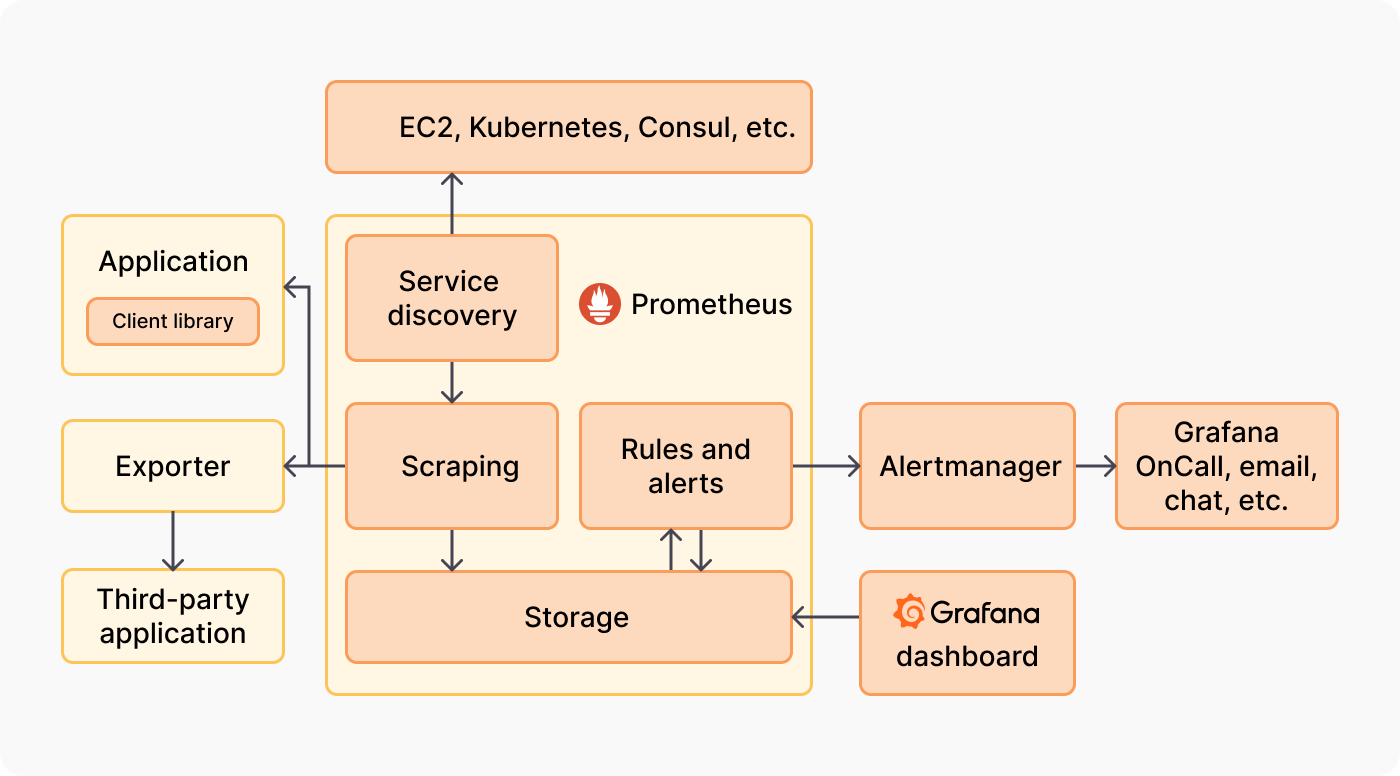
\includegraphics[width=16cm]{Figures/prometheus-grafana-architecture-diagram.png}
  \caption{Prometheus Architecture}
  \label{fig:prometheus_architecture}
\end{figure}

Figure \ref{fig:prometheus_architecture} illustrates the Prometheus architecture. Prometheus discovers targets to scrape via service discovery, which can include instrumented applications or third-party applications accessed through exporters. Scraped data is stored and can be utilized for dashboards using PromQL or for sending alerts to the Alertmanager, which converts them into various notifications.

\begin{itemize}
  \item \textbf{Client Libraries:} Client libraries allow for easy instrumentation of applications, typically requiring only a few lines of code. Prometheus provides official client libraries in Go, Python, Java/JVM, Ruby, and Rust, with third-party libraries available for other languages. These libraries handle thread safety, bookkeeping, and producing the Prometheus text format. They can automatically pick up metrics from dependencies and offer built-in metrics for CPU usage and garbage collection.
  
  \item \textbf{Exporters:} Exporters collect metrics from software that cannot be instrumented directly. They transform data from an application's metrics interface into the Prometheus exposition format. Exporters are widely available and can be easily extended if necessary.
  
  \item \textbf{Service Discovery:} Prometheus uses service discovery to locate and monitor applications and exporters. Integrations are available for Kubernetes, EC2, Consul, and more. Service discovery information is mapped to monitoring targets and their labels using relabeling.
  
  \item \textbf{Scraping:} Prometheus fetches metrics by sending HTTP requests called scrapes. The responses are parsed and stored. Scraping is configured to occur regularly, typically every 10 to 60 seconds per target.
  
  \item \textbf{Storage:} Prometheus stores data locally in a custom database, optimized for high performance. The storage system in Prometheus 2.0 can ingest millions of samples per second with efficient compression.
  
  \item \textbf{Dashboards:} Prometheus provides HTTP APIs for querying and displaying data. Grafana is recommended for creating advanced dashboards, supporting multiple Prometheus servers.
  
  \item \textbf{Recording Rules and Alerts:} Recording rules allow regular evaluation of PromQL expressions, storing the results. Alerting rules work similarly, generating alerts sent to the Alertmanager.
  
  \item \textbf{Alert Management:} The Alertmanager handles alerts from Prometheus servers, converting them into notifications via email, chat applications, and services like PagerDuty. Alerts can be aggregated, throttled, and routed based on different team requirements.
  
  \item \textbf{Long-Term Storage:} Prometheus stores data locally, limiting retention to available disk space. For long-term storage, remote read and write APIs enable integration with external systems for extended data retention.
\end{itemize}



\section{Grafana}

  
\begin{figure}[H]
  \centering
  
\includegraphics[width=5cm]{Logos/grafana-logo.png}
  \caption{Grafana}
\end{figure}
Grafana is an open-source analytics and visualization platform commonly used alongside Prometheus for monitoring and observability purposes.
Grafana provides a rich set of features for creating interactive dashboards and visualizations from various data sources, including Prometheus metrics, logs, and other time series databases.

\begin{itemize}
  \item \textbf{Dashboards:} With Grafana, users can easily create and customize dashboards to visualize key performance indicators, monitor system health, and track application metrics in real-time.
  \item \textbf{Visualization Options:} Grafana supports a wide range of visualization options, including graphs, tables, heatmaps, and histograms, allowing for flexible and insightful data analysis.
  \item \textbf{Integration:} Grafana offers extensive integration capabilities with numerous data sources, including Prometheus, Elasticsearch, Graphite, and InfluxDB, making it a versatile tool for consolidating and visualizing data from different sources in a single interface.
  \item \textbf{Advanced Features:} Grafana provides advanced features such as alerting and annotations, allowing users to set up alerts based on predefined thresholds or conditions and annotate dashboards with contextual information for improved situational awareness.
\end{itemize}

\section{Project Management Tool}

With the rapid evolution of information and communication technologies, user needs are increasing and becoming more demanding, while the economic context is constantly changing. In this context, managing IT projects has become a challenge for companies, as it is essential to master and successfully complete them, regardless of their size or type. For our DevSecOps team, which adopts the Agile Scrum method, Jira Software offers ready-to-use Scrum and Kanban boards. These boards serve as task management centers, where tasks are associated with customizable workflows. They ensure transparency of teamwork and provide visibility into the progress of each task. Time tracking features and real-time performance reports (Burnup/Burndown charts, sprint reports, velocity charts) allow the team to closely monitor its productivity over time.

\begin{figure}[h]
    \centering
    
\includegraphics[width=0.5\textwidth]{Logos/jira-png.png}
    \caption{Jira logo}
\end{figure}

\section{Conclusion}

Throughout this chapter, we have synthesized the selection of various tools necessary for the implementation of our project. By comparing the tools that correspond to our needs, we can detail the phases of implementing these solutions in the next chapter with the goal of achieving our objectives.

\pagebreak